\documentclass[12pt]{article}
\usepackage[a4paper,margin=0.75in]{geometry}
\usepackage[utf8]{inputenc}
\usepackage[OT1]{fontenc}
\usepackage[table,usenames,dvipsnames]{xcolor}
\usepackage{array}
\usepackage{varwidth}
\usepackage{tabularx}
\usepackage{amsmath}
\usepackage{hyperref}
\usepackage{enumitem}
\usepackage{graphicx}
\usepackage{tcolorbox}
\graphicspath{A2images/}
\renewcommand*\familydefault{\sfdefault}

\newtcolorbox{mybox}[3][]
{
  colframe = #2!25,
  colback  = #2!10,
  coltitle = #2!20!black,  
  title    = {#3},
  #1,
}

\hypersetup{
    colorlinks=true,
    linkcolor=blue,
    filecolor=magenta,      
    urlcolor=cyan,
    pdftitle={Overleaf Example},
    pdfpagemode=FullScreen,
}

\title{\textbf{COL774 Assignment 2}}
\author{Brian Sajeev Kattikat \\ \texttt{2021CS50609}}
\date{October 2023}

\begin{document}

\maketitle

\section{Naive }

\begin{enumerate}[label=(\alph*)]

    \item Naive Bayes was implemented using Multinoulli model.
          \begin{enumerate}[label=\roman*.]
              \item
                    \begin{itemize}
                        \item Accuracy in training set = 85.05\%                \item Accuracy in validation set = 67.05\%
                    \end{itemize}
              \item Word clouds for each class:
          \end{enumerate}
          \begin{center}
              \begin{tabular}{c c c}
                  
\includegraphics[width=0.3\textwidth]{Images/Q1/a/ptext.png} & \includegraphics[width=0.3\textwidth]{Images/Q1/a/neutext.png} &
                  
\includegraphics[width=0.3\textwidth]{Images/Q1/a/ntext.png}                                                                             \\
                  Positive                                                     & Neutral                                                        & Negative
              \end{tabular}
          \end{center}

    \item For random guessing, accuracy obtained was 32.13 \%, which is close to expected value of 33.33\%. For always predicting positive, the accuracy is 43.85\%, which would just simply show the percentage of positive tweets in the test data.

          The Part a) of Naive Bayes gives 109\% improvement over random guessing, and gives 52.91\% gain over always predicting positive.

    \item \begin{itemize}
              \item The confusion matrices for training set are as follows:
                    \begin{center}
                        \begin{tabular}{c c}
                            NaiveBayes                    & Random \\
                            \begin{tabular}{r|c|c|c}
                                    & AP    & ANu  & AN    \\
                                \hline
                                PP  & 15711 & 2158 & 1078  \\
                                \hline
                                PNu & 177   & 3574 & 171   \\
                                \hline
                                PN  & 714   & 1364 & 12917 \\
                                \hline
                            \end{tabular} &
                            \begin{tabular}{r|c|c|c}
                                    & AP   & ANu  & AN   \\
                                \hline
                                PP  & 5582 & 2381 & 4702 \\
                                \hline
                                PNu & 5464 & 2372 & 4727 \\
                                \hline
                                PN  & 5556 & 2343 & 4737 \\
                                \hline
                            \end{tabular}
                        \end{tabular}
                    \end{center}
                    \begin{center}
                        \begin{tabular}{c}
                            All Positive \\
                            \begin{tabular}{r|c|c|c}
                                    & AP    & ANu  & AN    \\
                                \hline
                                PP  & 16602 & 7096 & 14166 \\
                                \hline
                                PNu & 0     & 0    & 0     \\
                                \hline
                                PN  & 0     & 0    & 0     \\
                                \hline
                            \end{tabular}
                        \end{tabular}
                    \end{center}
              \item The confusion matrices for validation set are as follows:
                    \begin{center}
                        \begin{tabular}{c c}
                            NaiveBayes                & Random \\
                            \begin{tabular}{r|c|c|c}
                                    & AP   & ANu & AN  \\
                                \hline
                                PP  & 1197 & 338 & 305 \\
                                \hline
                                PNu & 21   & 101 & 17  \\
                                \hline
                                PN  & 226  & 178 & 910 \\
                                \hline
                            \end{tabular} &
                            \begin{tabular}{r|c|c|c}
                                    & AP  & ANu & AN  \\
                                \hline
                                PP  & 471 & 200 & 410 \\
                                \hline
                                PNu & 514 & 213 & 417 \\
                                \hline
                                PN  & 459 & 204 & 405 \\
                                \hline
                            \end{tabular}
                        \end{tabular}
                    \end{center}
                    \begin{center}
                        \begin{tabular}{c}
                            All Positive \\
                            \begin{tabular}{r|c|c|c}
                                    & AP   & ANu & AN   \\
                                \hline
                                PP  & 1444 & 617 & 1232 \\
                                \hline
                                PNu & 0    & 0   & 0    \\
                                \hline
                                PN  & 0    & 0   & 0    \\
                                \hline
                            \end{tabular}
                        \end{tabular}
                    \end{center}
          \end{itemize}


          We can show that the Naive Bayes classifier has much higher accuracy than random guessing or constant classification.

    \item The following transformations were done in order:
          \begin{itemize}
              \item Convert HTML references to unicode, i.e. convert "\&amp;" to \&, "\&lt;" to \< etc.
              \item convert to lowercase.
              \item remove non-ascii characters.
              \item remove links and @tags.
              \item Tokenize to extract only alphanumeric and ' values.
              \item remove stopwords.
              \item Lemmatize.
          \end{itemize}

          \begin{center}
              \begin{center}
                  \begin{tabular}{c c c}
                      
\includegraphics[width=0.3\textwidth]{Images/Q1/d/ptext.png} & \includegraphics[width=0.3\textwidth]{Images/Q1/d/neutext.png} &
                      
\includegraphics[width=0.3\textwidth]{Images/Q1/d/ntext.png}                                                                             \\
                      Positive                                                     & Neutral                                                        & Negative
                  \end{tabular}
              \end{center}
          \end{center}

          The output accuracy produced was:
          \begin{itemize}
              \item Naive Bayes prediction accuracy with stemming = 69.85\%
              \item Naive Bayes prediction accuracy with lemmatizing = 70.91\%
          \end{itemize}

          Observations:
          \begin{itemize}
              \item Accuracy increased because after cleaning there is lesser noise in the data.
              \item Lemmatizing seems to have better accuracy and performance over stemming.
          \end{itemize}



    \item Bigrams has not been implemented:
          % Using Bigrams (in addition to removing stopwords and stemming) gives us an accuracy of \textbf{84.4 \%}, with 8209/10000 positive reviews and 4447/5000 negative reviews correctly classified.

          %     For the additional feature, we use Trigrams. Using trigrams, in addition to bigrams and removing stopwords + stemming gives us an accuracy of \textbf{85.2 \%}, with 8352/10000 positive reviews and 4423/5000 negative reviews correctly classified.

          %     The additional sets of features do help us improve our accuracy (explain why)

    \item Using Domain adaptation the following results were obtained:

          \begin{enumerate}[label=\roman*.]
              % \item Using Source Data:
              \begin{itemize}

                  % \item The prediction accuracy when using split 1 with source domain is 47.97879390324719
                  % \item The prediction accuracy when using split 2 with source domain is 48.31013916500994
                  % \item The prediction accuracy when using split 5 with source domain is 48.70775347912525
                  % \item The prediction accuracy when using split 10 with source domain is 50.132538104705105
                  % \item The prediction accuracy when using split 25 with source domain is 50.56328694499669
                  % \item The prediction accuracy when using split 50 with source domain is 51.789264413518886
                  % \item The prediction accuracy when using split 100 with source domain is 54.208084824387015 
              \end{itemize}
              % \item Without using Source Data:
              \begin{itemize}
                  % \item The prediction accuracy when using split 1 is 34.327369118621604
                  % \item The prediction accuracy when using split 2 is 35.387673956262425
                  % \item The prediction accuracy when using split 5 is 39.72829688535454
                  % \item The prediction accuracy when using split 10 is 44.26772697150431
                  % \item The prediction accuracy when using split 25 is 46.02385685884692
                  % \item The prediction accuracy when using split 50 is 49.07223326706428
                  % \item The prediction accuracy when using split 100 is 52.51822398939695
                  \item For size 1%
                  \item combined with corona tweets:
                  \item Accuracy:0.43240556660039764
                  \item Without corona tweets
                  \item Accuracy:0.3465871438038436
                  \item For size 2%
                  \item combined with corona tweets:
                  \item Accuracy:0.43538767395626243
                  \item Without corona tweets
                  \item Accuracy:0.35155732273028495
                  \item For size 5%
                  \item combined with corona tweets:
                  \item Accuracy:0.4469847581179589
                  \item Without corona tweets
                  \item Accuracy:0.41583830351225975
                  \item For size 10%
                  \item combined with corona tweets:
                  \item Accuracy:0.46421471172962225
                  \item Without corona tweets
                  \item Accuracy:0.44532803180914515
                  \item For size 25%
                  \item combined with corona tweets:
                  \item Accuracy:0.48111332007952284
                  \item Without corona tweets
                  \item Accuracy:0.4486414844267727
                  \item For size 50%
                  \item combined with corona tweets:
                  \item Accuracy:0.4993373094764745
                  \item Without corona tweets
                  \item Accuracy:0.4854208084824387
              \end{itemize}
              \item The obtained graph is as follows:
                    % \begin{center}\raisebox{-.9\height}{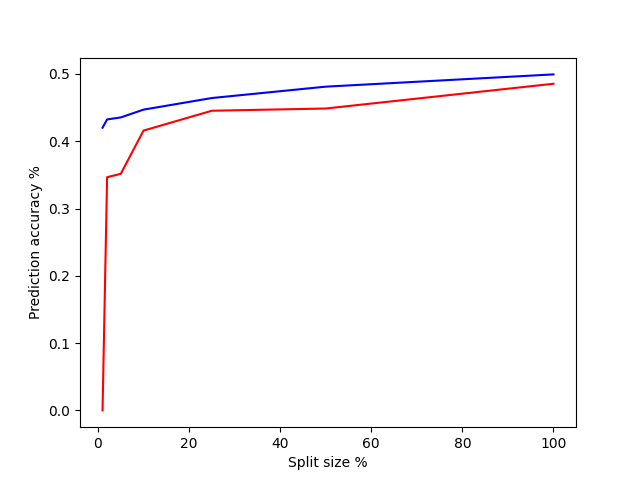
\includegraphics[width=0.7\textwidth]{Images/Q1/f/Source_vs_NoSource.png}}\end{center}
                    % \newpage
                    \end{itemize}
          \end{enumerate}


\end{enumerate}

\clearpage

\section{Binary SVM}

\begin{enumerate}[label=(\alph*)]
    \item \begin{enumerate}[label=\roman*.]
              \item For linear kernel, datasets 3 and 4,
                    \begin{itemize}
                        \item No of support vectors: 3066 out of 4760
                        \item \% of support vectors wrt training examples: 64.41\%
                    \end{itemize}
              \item The test accuracy we obtain is 71.00\%
              \item The top 6 support vectors are:

                    \begin{center}
                        \begin{tabular}{c c c}
                            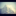
\includegraphics[width=0.2\textwidth{Images/Q2/CVXOPT_linear_top1.png}  &
                            \includegraphics[width=0.2\textwidth]{Images/Q2/CVXOPT_linear_top2.png} &
                            
\includegraphics[width=0.2\textwidth]{Images/Q2/CVXOPT_linear_top3.png}   \\
                        \end{tabular}
                        \begin{tabular}{c c c}
                            
\includegraphics[width=0.2\textwidth]{Images/Q2/CVXOPT_linear_top4.png} &
                            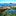
\includegraphics[width=0.2\textwidth]{Images/Q2/CVXOPT_linear_top5.png} &
                            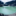
\includegraphics[width=0.2\textwidth]{Images/Q2/CVXOPT_linear_top6.png}   \\
                        \end{tabular}
                    \end{center}

                    The weight image obtained is:

                    \begin{center}
                        
\includegraphics[width=0.2\textwidth]{Images/Q2/CVXOPT_w_img.png}
                    \end{center}
          \end{enumerate}

    \item \begin{enumerate}[label=\roman*.]
              \item For gaussian kernel, datasets 3 and 4,
                    \begin{itemize}
                        \item No of support vectors: 3682 out of 4760
                        \item \% of support vectors wrt training examples: 77.35\%
                        \item No of common support vectors between linear and gaussian: 2895
                    \end{itemize}
              \item The test accuracy we obtain is 76.25\%
              \item The top 6 support vectors are:

                    \begin{center}
                        \begin{tabular}{c c c}
                            
\includegraphics[width=0.2\textwidth]{Images/Q2/CVXOPT_rbf_top1.png} &
                            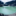
\includegraphics[width=0.2\textwidth]{Images/Q2/CVXOPT_rbf_top2.png} &
                            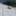
\includegraphics[width=0.2\textwidth]{Images/Q2/CVXOPT_rbf_top3.png}   \\
                        \end{tabular}
                        \begin{tabular}{c c c}
                            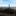
\includegraphics[width=0.2\textwidth]{Images/Q2/CVXOPT_rbf_top4.png} &
                            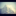
\includegraphics[width=0.2\textwidth]{Images/Q2/CVXOPT_rbf_top5.png} &
                            
\includegraphics[width=0.2\textwidth]{Images/Q2/CVXOPT_rbf_top6.png}   \\
                        \end{tabular}
                    \end{center}
              \item We can observer that gaussian kernel can get slightly more accuracy than linear kernel.
          \end{enumerate}

    \item \begin{enumerate}[label=\roman*.]
              \item Number of Support Vectors obtained, using sklearn's SVC:
                    \begin{itemize}
                        \item Linear Kernel: 2942, and 2942 SVs in common with CVXOPT version.
                        \item Gaussian Kernel: 3393, and 3393 SVs in common with CVXOPT version.
                        \item between both linear and gaussian there are 2722 common SVs.
                    \end{itemize}
                    % \begin{center}
                    %     \begin{tabular}{c c}
                    %         & CVXOPT \\
                    %         Scikit & 
                    %     \begin{tabular}{c|c|c|}
                    %             & lin  & rbf  \\   
                    %         \hline
                    %         lin & 669 & 569 \\
                    %         \hline
                    %         rbf & 566 & 1056 \\
                    %         \hline
                    %     \end{tabular}
                    %     \end{tabular}
                    % \end{center}

              \item Comparison of weight and bias in linear kernel:
                    \begin{itemize}
                        \item CVXOPT: b = -0.7401936386523351
                        \item sklearn\_svm: b = -0.80421845
                        \item norm(w\_cv - w\_skl) = 0.01106776175233239
                    \end{itemize}
              \item Validation set accuracy is as follows:
                    \begin{itemize}
                        \item Linear Kernel: sklearn\_svm obtains 71.50\% accuracy over CVXOPT's 71.00\% accuracy
                        \item Gaussian Kernel: sklearn\_svm obtains 76.75\% accuracy over CVXOPT's 76.25\% accuracy
                    \end{itemize}

              \item The training times are given below:
                    \begin{center}
                        \begin{tabular}{|l|c|}
                            \hline
                            Scikit RBF    & 3.99s  \\
                            Scikit linear & 6.96s  \\
                            CVXOPT RBF    & 51.67s \\
                            CVXOPT linear & 61.28s \\
                            \hline
                        \end{tabular}
                    \end{center}
          \end{enumerate}

\end{enumerate}

% \section{Multiclass SVM}

\end{enumerate}

\end{document}